% THIS IS SIGPROC-SP.TEX - VERSION 3.0
% WORKS WITH V3.1SP OF ACM_PROC_ARTICLE-SP.CLS
% JUNE 2007
%
% It is an example file showing how to use the 'acm_proc_article-sp.cls' V3.1SP
% LaTeX2e document class file for Conference Proceedings submissions.
% ----------------------------------------------------------------------------------------------------------------
% This .tex file (and associated .cls V3.1SP) *DOES NOT* produce:
%       1) The Permission Statement
%       2) The Conference (location) Info information
%       3) The Copyright Line with ACM data
%       4) Page numbering
% ---------------------------------------------------------------------------------------------------------------
% It is an example which *does* use the .bib file (from which the .bbl file
% is produced).
% REMEMBER HOWEVER: After having produced the .bbl file,
% and prior to final submission,
% you need to 'insert'  your .bbl file into your source .tex file so as to provide
% ONE 'self-contained' source file.
%
% Questions regarding SIGS should be sent to
% Adrienne Griscti ---> griscti@acm.org
%
% Questions/suggestions regarding the guidelines, .tex and .cls files, etc. to
% Gerald Murray ---> murray@acm.org
%
% For tracking purposes - this is V3.0SP - JUNE 2007

\documentclass{acm_proc_article-sp}
\usepackage{ae,aecompl}
\usepackage{wrapfig}
\usepackage{subfigure}

\begin{document}

\title{Facial Detection and Stereo Localization}
%\subtitle{[Extended Abstract]
%\titlenote{A full version of this paper is available as
%\textit{Author's Guide to Preparing ACM SIG Proceedings Using
%\LaTeX$2_\epsilon$\ and BibTeX} at
%\texttt{www.acm.org/eaddress.htm}}}

% You need the command \numberofauthors to handle the 'placement
% and alignment' of the authors beneath the title.
%
% For aesthetic reasons, we recommend 'three authors at a time'
% i.e. three 'name/affiliation blocks' be placed beneath the title.
%
% NOTE: You are NOT restricted in how many 'rows' of
% "name/affiliations" may appear. We just ask that you restrict
% the number of 'columns' to three.
%
% Because of the available 'opening page real-estate'
% we ask you to refrain from putting more than six authors
% (two rows with three columns) beneath the article title.
% More than six makes the first-page appear very cluttered indeed.
%
% Use the \alignauthor commands to handle the names
% and affiliations for an 'aesthetic maximum' of six authors.
% Add names, affiliations, addresses for
% the seventh etc. author(s) as the argument for the
% \additionalauthors command.
% These 'additional authors' will be output/set for you
% without further effort on your part as the last section in
% the body of your article BEFORE References or any Appendices.

\numberofauthors{3} %  in this sample file, there are a *total*
% of EIGHT authors. SIX appear on the 'first-page' (for formatting
% reasons) and the remaining two appear in the \additionalauthors section.
%
\author{
% You can go ahead and credit any number of authors here,
% e.g. one 'row of three' or two rows (consisting of one row of three
% and a second row of one, two or three).
%
% The command \alignauthor (no curly braces needed) should
% precede each author name, affiliation/snail-mail address and
% e-mail address. Additionally, tag each line of
% affiliation/address with \affaddr, and tag the
% e-mail address with \email.
%
% 1st. author
\alignauthor
David Litwak\\
       \affaddr{University of California at Berkeley}\\
       \email{dlitwak@berkeley.edu}
% 2nd. author
\alignauthor
Timothy Liu\\
       \affaddr{University of California at Berkeley}\\
       \email{timothytliu@berkeley.edu}
% 3rd. author
\alignauthor
Jens Tyge Tiessen\\
       \affaddr{University of California at Berkeley}\\
       \email{ttiessen@berkeley.edu}
}

\maketitle
\begin{abstract}
This paper presents an innovative setup for facial recognition. The system uses 3 cameras to perform stereo localization and combines front and profile face detection with a skin filter and contour analysis to recognize faces. It then combines localization with facial detection to give a person his or her orientation by highlighting the camera with the better view of the person.
\end{abstract}

\terms{Stereo Calibration, Viola-Jones Algorithm, Hough Circles}

\keywords{Center of Mass, Localization, Face Detection, Orientation, Threading} % NOT required for Proceedings

\section{Introduction}
The goal of this experiment was to facilitate facial recog- nition in any environment. Facial recognition requires an optimal view of the face and recognition itself can be very unreliable. Moving targets can move away from a camera's perspective and the surroundings can produce false positives. Therefore, multiple cameras can provide a dynamic and adaptive field of view, and stereo localization can help tune the location of targets. This experiment provided results for a three camera system that triangulated target position and detected faces. Together the two provided a 
highlighted camera view of the camera with the best orientation 
or probability that a face would be recognized.

\section{Project Components and Setup}

\subsection{Hardware and Software}
The basis of the experiment revolved around these hardware and software components.
\begin{itemize}
\item 3 Logitech QuickCam Pro for Notebooks
\item 3 16 ft. USB-to-USB Cables
\item 3 6 ft. wire stands
\end{itemize}

\begin{itemize}
\item OpenCV \footnote{http://sourceforge.net/projects/opencvlibrary}
\item VideoInput \footnote{http://muonics.net/school/spring05/videoInput/}
\item Camera Calibration \footnote{http://www.vision.caltech.edu/bouguetj/calib\_doc/}
\item Visual C++ 2008 Express \footnote{http://www.microsoft.com/express/vc/}
\end{itemize}

However, these simple components had very little in common, especially the two vision libraries with three cameras.
Initially, software had to be modified greatly as OpenCV could not interface with more than two USB cameras nor change to higher resolution.
Also, resolution was extremely important because faces would decrease in size at further distances.  VideoInput allowed for
easier video acquisition, multiple cameras, dynamic frame rate, and resizable resolution.  The OpenCV library, however, contained a multitude of functions
ranging from machine learning, simple image processing, and stereo camera functions.

A majority of the software modifications involved interfacing between different image objects(unsigned char * vs. IplImage *), 
different image formats (BGR flipped vertifcal vs. RGB), and different GUI displays (1 OpenGL window vs. many Image Windows).
Furthermore, using both OpenCV and VideoInput libraries required a multitude of dependencies including Windows SDK, Windows DirectShow, etc.
It would be more beneficial to understand and commit to a specific image processing library and then choose relevant hardware setup.

\subsection{Setup}
The experiment required a very stable and controlled environment.  The setup included mounting each webcamera on top of the wire stands.
After positioning the wire stands and cameras in a specific location, the cameras should not move at all.  
This is due to the calibration of the cameras, which would be incorrect if the camers moved.  The ideal setup for this experiment positions
three cameras at three vertices of a square.  The three cameras' focal length projection should ideally intersect at one point.  The fourth vertex simulates the doorway or area of entrance for the target.  This helps to generate the largest field of view for this experiment.  See Figure 1.

	\begin{figure}
		\centering
		\subfigure[Setup]{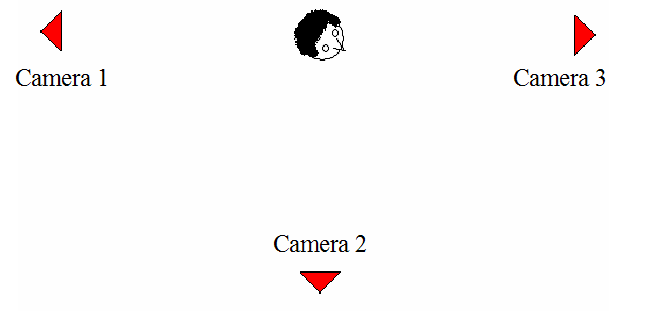
\includegraphics[width=0.3\textwidth]{setup.png}}\hfill
		\caption{\label{fig:setup}Picture of Hardware Setup}
	\end{figure}

\section{Project Design}
The project design focused on utilizing two known concepts to improve on a third.
The design focused on completing localization of faces, then detection of faces.  Afterwards,
combine the metadata obtained from both algorithms to produce something useful in discovering the target and its orientation.

\subsection{Localization}
The localization process consists of three major parts. Firstly, the cameras have to be calibrated so that the focal lengths and the relative positions and orientations of the cameras are known. Secondly, the object of interest has to be detected in the images. Finally, putting those informations together, we obtain the position of the object in a triangulation process.

Initially we wanted to implement the calibration functions ourself. After reading through the relevant chapters of "Invitation to 3D-Vision", we realized though that the easiest algorithm (the so-called "eight-point-algorithm") would already be quite a bit of work to implement in C++ without delivering good results and being very robust. We therefore decided to use the Matlab calibration tool that we already used in the labs and transfer the results manually to our program. As the checkers boards used in class were to small for the distances at which we used the cameras, we used a picture frame instead that measured about 30 by 25 inches. We calculated the rotation matrices and translation vectors for the left camera and the middle camera as will as the middle camera and the right camera.

For the detection of the target person in the image, we decided to a center of mass calculation. As we did not want to rely on an unvarying background, we decided to use a difference algorithm instead. In the first step, we take the absolute difference of two consecutive images of the video stream. The resulting image is then being filtered with a threshold, eliminating noise effects in the image.\\
An edge detection algorithm is now being used to find the edges of any moving objects and the result is then being smoothed with a Gaussian functioned. To tell the target person apart from other potentially moving objects in the image, we apply an algorithm that finds and lists any contours it can find in the image. To decide which contour corresponds to the target person, we simply choose the biggest contour. We then calculate the center of mass for this contour and use that as our target position in the image.

For the triangulation, we use the rotation matrices and translation vectors obtained in the triangulation process to calculate the lines generated by the positions in the image. As in 3D-space those lines normally do not intersect we assume that the cameras are all parallel to the ground and reduce the problem to a two dimensional problem. We triangulate with both pairs of cameras for which we did the calibration. Thus we obtain the position of the target with two independent ways.

As we use the left camera as the reference frame, we apply the rotation matrices and translation vectors again to determine the positions and orienation of the other cameras in that frame. Together with the two results from the triangulation we display those results on the screen. Depending on the camera setup, we adjust the scaling such that it fits into our frame.

\subsection{Face Detection}
The initial concept for face detection focused on finding specific face features within an image.  
However, an implemented algorithm proved to be more convenient because face detection was not the final goal.  
Therefore, the OpenCV library contained a face detection function using the Viola-Jones algorithm\footnote{http://prism2.mem.drexel.edu/~paul/openCv/openCvPart02.pdf}.
This algorithm detects Haar-like features (edges, lines, centers) and chooses which areas that are most likely faces.
	
The design required to detect faces in any kind of orientation.  This meant that multiple cascades of the face detection algorithm had to be used.
Three cascades were chained together: default front-face(agressive), alternative front-face(passive), and profile cascade.  
However, this was extremely computer intensive and the implemented Viola-Jones algorithm proved to be somehwat unreliable.  
If most faces were detected, then false positives were also detected.  If the false positives were tuned down, too few faces were properly detected.  
A design decision was made to try to identify most faces including false positives.
Post-processing of the detected rectangles would eliminate some if not most of the false positives.

The first method attempted was a skin filter\footnote{www.hpl.hp.com/techreports/Compaq-DEC/CRL-98-11.pdf}.
A skin filter looks at a given area of an image and computes the probability of whether or not it is a face.
This is accomplished by summing the probability of each pixel being skin given its color value.  
This can be expressed in the equations below.
\begin{equation}
\label{eq:skinfilter1}
P(rgb|skin) = \frac{s[rgb]}{T_s}, P(rgb|\neg skin) = \frac{n[rgb]}{T_n}
\end{equation}
\begin{equation}
\label{eq:skinfilter2}
P(skin|rgb) = \frac{P(rgb|skin)P(skin)}{P(rgb|skin)P(skin) + P(rgb|\neg skin)P(\neg skin)}
\end{equation}
Specifically, $P(skin|rgb) \geq \theta$ defines when a pixel is labeled skin.  To compensate
for luminosity, chromatic colors are used: $r\ or\ g\ or\ b\ =\ \frac{R\ or\ G\ or\ B}{R+G+B}$.  

Another method used to eliminate false positives was to subtract motionless areas from the background.
This enabled the detection algorithm to run more efficiently.
This method followed the following steps:
\begin{enumerate}
\item Differencing Algorithm (See Figure 2a)
\item Thresholding and Smoothing
\item Calculate Hough Circles
\item Create a mask from the Hough Circles
\item Mask the original image with the mask (See Figure 2c)
\item Remaining image keeps only whats in the circles
\end{enumerate}
However, this method was later replaced by a different motion detection algorithm (after calculating center of mass) 
because it required too much processing. Finding the hough circles of a grayscale image even after differencing and 
thresholding was too computer intensive. The frame rate was lowered to 10fps, but face detection hadn't even run yet.

	\begin{figure}
		\subfigure[Differencing Algorithm]{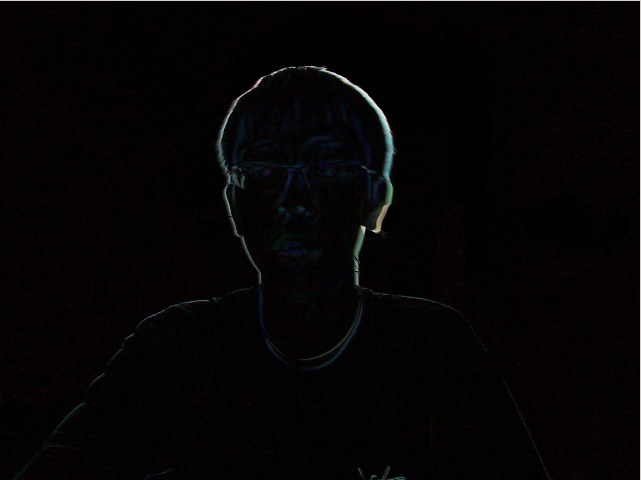
\includegraphics[width=0.2\textwidth]{diff.png}}\hfill
		\subfigure[Edge Detection Algorithm]{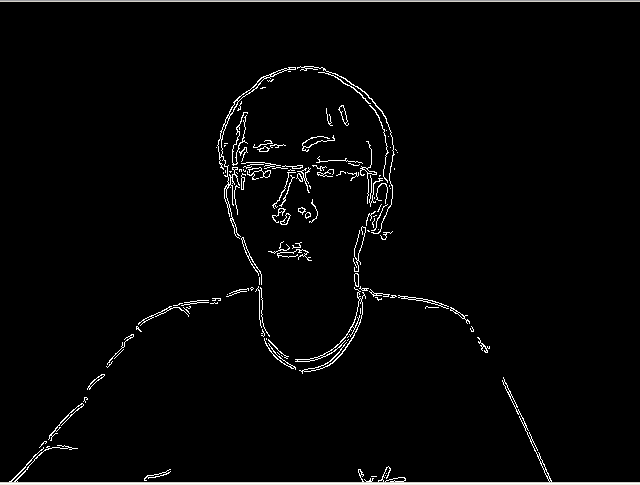
\includegraphics[width=0.2\textwidth]{edge.png}}\hfill
		\subfigure[Background Subtraction]{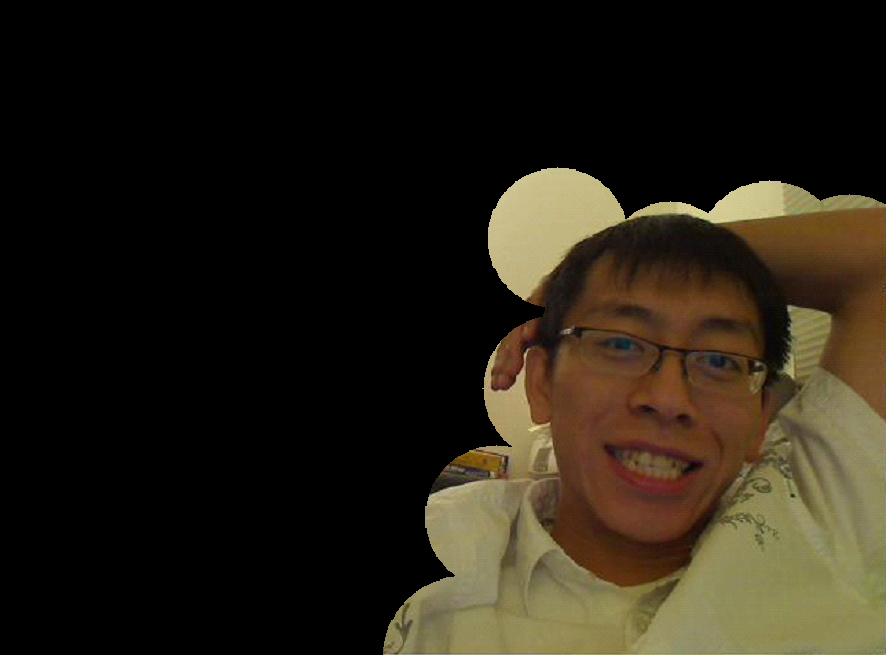
\includegraphics[width=0.2\textwidth]{motion.png}}\hfill
		\subfigure[Face Detection]{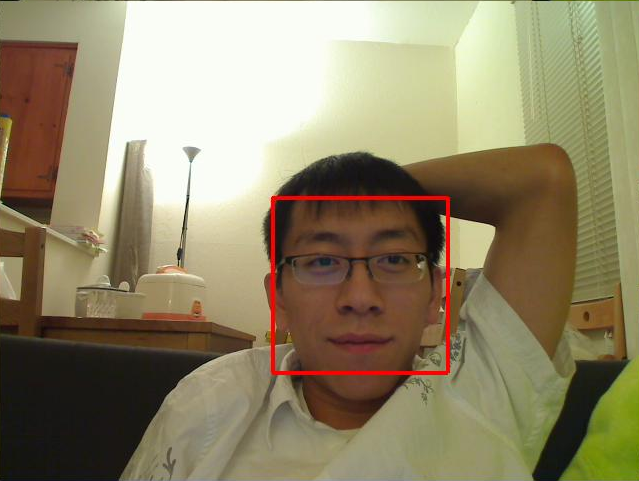
\includegraphics[width=0.2\textwidth]{detect.png}}\hfill
		\caption{\label{fig:detection} Face detection}
	\end{figure}
	
\subsection{Target Recognition and Orientaton}
To identify the orientation of the target persons face, we try to get rid of the last false positives of the face detection by only removing all results that do not share the same x-coordinates as the detected contour. As the face detection algorithm does not work very reliable and tends to detect the same face several times, we choose the camera that has the best frontal view on the face by choosing the one that detects the most frontal faces. Combining this with the detection of profiles this can then be used to estimate the orientation of the face.

\section{Project Results}
\subsection{Localization}
The localization worked very good as long as the target was moving and staying inside the range of the cameras. Both independently calculated positions were then overlapping or very close. But if the target moved out of side of one of the cameras, stood still or another person entered the space, the detected points could be quite a bit apart - an indication of an error in the localization.  See Figure 3.

In the process of localization there are several sources of error. Although we optimized the process of finding the position of the target person in the images, the process of calculating the center of mass is intrinsically prone deliver two positions that might not correspond to each other. Also, multiple persons in the camera range can mess up the whole calculation as the algorithm only associates the biggest contours with each other although they might not  be related. It was not possible with a reasonable amount of effort to get rid of this problem as a solution would have involved combining many consecutive calculations to establish correlation matrices.

	\begin{figure}
		\centering
		\subfigure[Contours]{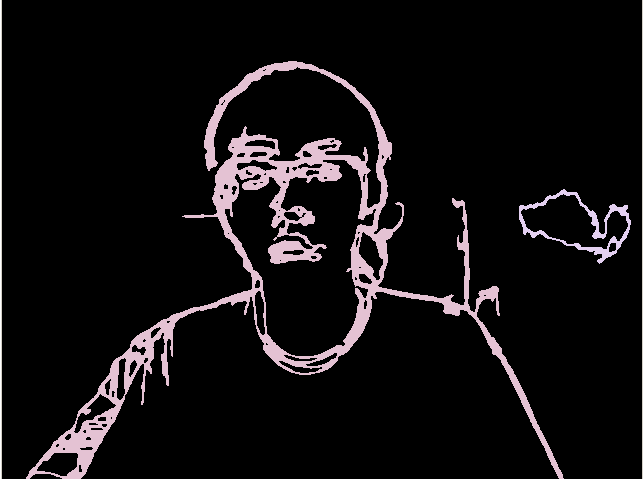
\includegraphics[width=0.3\textwidth]{contour.png}}\hfill
		\caption{\label{fig:contour}Contours to calculate center of mass}
	\end{figure}

	\begin{figure}
		\centering
		\subfigure[Localization]{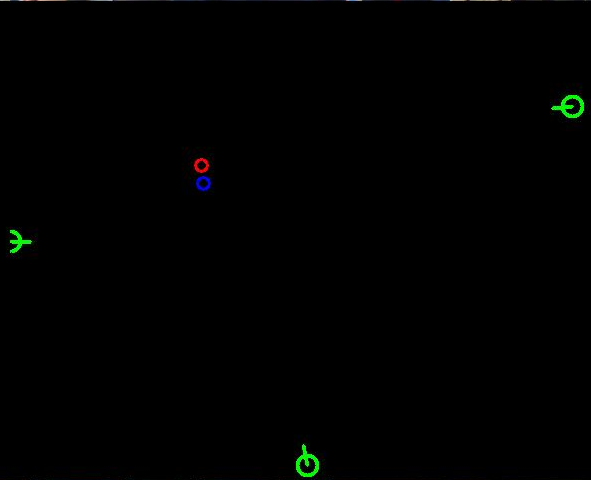
\includegraphics[width=0.3\textwidth]{localization.png}}\hfill
		\caption{\label{fig:localization}Localization with Three Cameras}
	\end{figure}

\subsection{Face Detection}
A sample of the results of face detection can be seen in Figure 5.  However, face detection remained extremely unreliable, which is also seen in Figure 5.
Overall, the results were adequate.  By applying several algorithms to reduce the number of false positives, faces were accurately detected.  The main issue
involved with facial detection was the amount of time spent processing and a colorful background.  A single call to face detection would decrease the frame rate
down to 2 frames per second.  If the experiment was to continue, a solution would have to be found.  See Figure 4 and Figure 5 for resulting pictures.

Threading proved to be the solution to the problem.  The experiment currently spawns three threads to calculate center of mass and triangulation.  Six threads are 
spawned to face detect: three for front-face and three for profile face detection.  Now, the frame rate can go from 5 frames per second up to 20 frames per second.  
This is a significant increase in the quality of processing and presentation.  As for the solution to the colorful background, both center of mass and background
subtraction are possible solutions.  The final presentation of this experiment simply controlled the environment placing the background as all white.

	\begin{figure}
		\centering
		\subfigure[Correct Face detection]{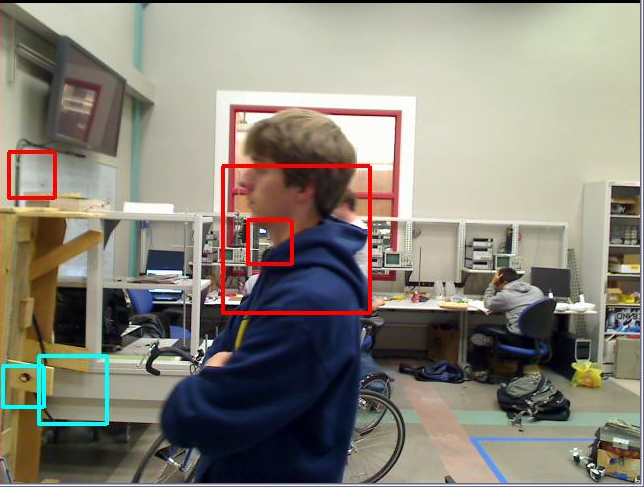
\includegraphics[width=0.3\textwidth]{facedetect.png}}\hfill
		\subfigure[Incorrect Face detection]{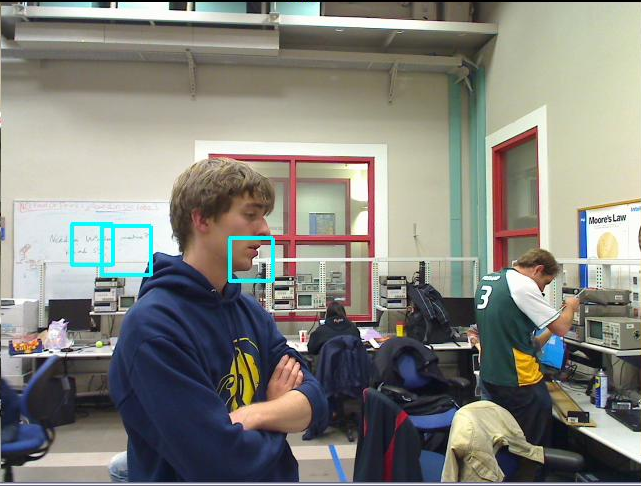
\includegraphics[width=0.3\textwidth]{unreliable.png}}\hfill
		\caption{\label{fig:profileface}Correct and Incorrect Facial Detection}
	\end{figure}

\subsection{Target Recognition and Orientaton}
As the face detection did not nearly work as reliable as we hoped it would, we had to fight with very low detection rates and quite a lot of false positives that we could not completely get rid of despite the use of several different methods to reduce the impact of the background and noise. It also happened often that a profile was detected as a frontal face and vice versa.

Thus the results of the detection of the actual orientation of the face were not very convincing. If the program would have been able to run faster the whole process might have improved too. But despite the use of threading, faces were detected only about every two to three seconds.  The final result can be seen in Figure 6.  Note that the center camera view has a highlighted box, which denotes the best camera position.

	\begin{figure}
		\centering
		\subfigure[Combined]{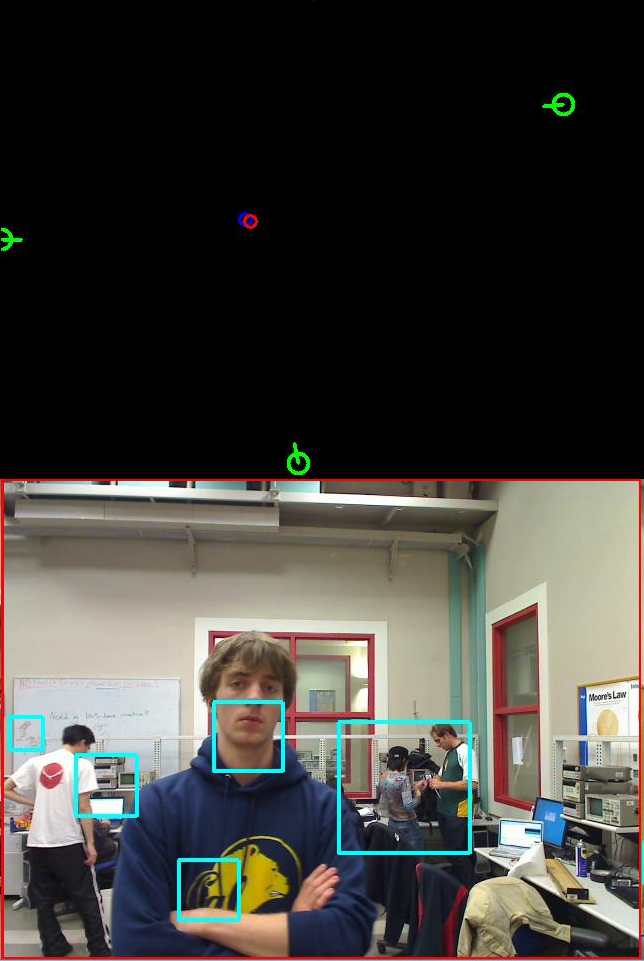
\includegraphics[width=0.3\textwidth]{combined.png}}\hfill
		\caption{\label{fig:Combined}Face Detection with highlighting Center of Mass}
	\end{figure}
		
\section{Conclusion}
We succeeded in accomplishing our goal of designing a 3-camera system that could effectively localize a moving object, detect a face, and combine the two to provide the subject with his or her orientation. Problems still persist though. Some are due to an unreliable facial detection algorithm. The system currently only supports one subject and becomes confused in the presence of two or more, altering the localization calculations and subsequently the orientation calculations. Threads solved some of our frame rate problems but speed can definitely be improved. But overall the project was a success. In a controlled environment with a single subject our system successfully performed localization, detection and orientation.

\section{Acknowledgments}
We'd like to thank Professor Ruzena Bajcsy, Edgar Lobaton, Yasemin Demir, and Winthrop for their great help with this project.

\section{References}
[1] Ma, Yi. Soatto, Stefano. Kosecka, Jana. Sastry, S. Shankar. An Invitation to 3D Vision. Springer Science + Business Media LLC. 2006.

[2] Jones, Michael and Rehg, James.  Statistical Color Models with Application to Skin Detection. Cambridge Research Laboratory. December 1998. www.hpl.hp.com/techreports/ Compaq-DEC/CRL-98-11.pdf

[3] Hewlett, Robin. Seeing with OpenCV: A Computer Vision Library. Servo Magazine. January 2007. http://prism2. mem.drexel.edu/$\sim$paul/openCv/openCvPart01.pdf
\balancecolumns
\end{document}
